%%%%%%%%%%%%%%%%%%%%%%%%%%%%%%%%%%%%%%%%%
% Academic Title Page
% LaTeX Template
% Version 2.0 (17/7/17)
%
% This template was downloaded from:
% http://www.LaTeXTemplates.com
%
% Original author:
% WikiBooks (LaTeX - Title Creation) with modifications by:
% Vel (vel@latextemplates.com)
%
% License:
% CC BY-NC-SA 3.0 (http://creativecommons.org/licenses/by-nc-sa/3.0/)
% 
% Instructions for using this template:
% This title page is capable of being compiled as is. This is not useful for 
% including it in another document. To do this, you have two options: 
%
% 1) Copy/paste everything between \begin{document} and \end{document} 
% starting at \begin{titlepage} and paste this into another LaTeX file where you 
% want your title page.
% OR
% 2) Remove everything outside the \begin{titlepage} and \end{titlepage}, rename
% this file and move it to the same directory as the LaTeX file you wish to add it to. 
% Then add \input{./<new filename>.tex} to your LaTeX file where you want your
% title page.
%
%%%%%%%%%%%%%%%%%%%%%%%%%%%%%%%%%%%%%%%%%

%----------------------------------------------------------------------------------------
%	PACKAGES AND OTHER DOCUMENT CONFIGURATIONS
%----------------------------------------------------------------------------------------

\documentclass[11pt]{article}

%%Packages

\usepackage{appendix}

%Matematiske
\usepackage{amsmath} %Blant annet referer til likninger
\usepackage{amsfonts} %Inneholder matematiske fonter mathbb
\usepackage{physics}


%Grafisk
\usepackage{graphicx}
\usepackage{subcaption}
\usepackage{float} %Brukes med H for å sette posisjon til figur
\usepackage{pythonhighlight}
\usepackage{listings}
\usepackage{xcolor} % for setting colors
\usepackage{setspace}

%Kommentar
\usepackage[colorinlistoftodos]{todonotes}

%Til hyperlinker
\usepackage[colorlinks=true, breaklinks]{hyperref}%Breaklink deler opp linken dersom for lang

\usepackage[utf8]{inputenc} % Required for inputting international characters
\usepackage[T1]{fontenc} % Output font encoding for international characters

\usepackage{baskervillef} % Palatino font

% kode
\usepackage[ruled,vlined]{algorithm2e}
\lstset { %
	language=C++,
	backgroundcolor=\color{black!5}, % set backgroundcolor
	basicstyle=\footnotesize,% basic font setting
}



\begin{document}
	%----------------------------------------------------------------------------------------
	%	TITLE PAGE
	%----------------------------------------------------------------------------------------
	
	\begin{titlepage} % Suppresses displaying the page number on the title page and the subsequent page counts as page 1
		\newcommand{\HRule}{\rule{\linewidth}{0.5mm}} % Defines a new command for horizontal lines, change thickness here
		
		\center % Centre everything on the page
		
		%------------------------------------------------
		%	Headings
		%------------------------------------------------
		
		\textsc{\LARGE University of Oslo}\\[1.5cm] % Main heading such as the name of your university/college
		
		\textsc{\Large FYS3150}\\[0.5cm] % Major heading such as course name
		
		\textsc{\large Computational Physics}\\[0.5cm] % Minor heading such as course title
		
		%------------------------------------------------
		%	Title
		%------------------------------------------------
		
		\HRule\\[0.4cm]
		
		{\huge\bfseries Eigensolvers \\ A Numerical Study of Eigenvalue Problems}\\[0.4cm] % Title of your document
		
		\HRule\\[1.5cm]
		
		%------------------------------------------------
		%	Author(s)
		%------------------------------------------------
		
		%	\begin{minipage}{0.4\textwidth}
		%		\begin{flushleft}
		%			\large
		%			\textit{Author}\\
		%			B.J. \textsc{Blazkowicz} % Your name
		%		\end{flushleft}
		%	\end{minipage}
		%	~
		%	\begin{minipage}{0.4\textwidth}
		%		\begin{flushright}
		%			\large
		%			\textit{Supervisor}\\
		%			Dr. Caroline \textsc{Becker} % Supervisor's name
		%		\end{flushright}
		%	\end{minipage}
		
		% If you don't want a supervisor, uncomment the two lines below and comment the code above
		{\large\textit{Authors}}\\
		\textsc{Lars Kristian Skaar}\\\textsc{Brage Brevig} % Your name
		\\
		\url{https://github.uio.no/lkskaar/FYS3150}
		%------------------------------------------------
		%	Date
		%------------------------------------------------
		
		\vfill\vfill\vfill % Position the date 3/4 down the remaining page
		
		{\large\today} % Date, change the \today to a set date if you want to be precise
		
		%------------------------------------------------
		%	Logo
		%------------------------------------------------
		
		\vfill\vfill
		%
\includegraphics[width=0.5\textwidth]{logouio.png}\\[6cm] % Include a department/university logo - this will require the graphicx package
		
		%----------------------------------------------------------------------------------------
		
		%\vfill % Push the date up 1/4 of the remaining page
		
	\end{titlepage}

	%----------------------------------------------------------------------------------------
	\newpage
	\setstretch{1.5}
	\setlength\parindent{0pt}
	\section{Abstract}
	In this numerical project, we study the Jacobi Rotation Method as an eigenvalue solver. We then devise this solver to study different physical systems. We find that the Jacobi Rotation Method is an inefficient, yet precise eigenvalue solver wherein we have found that the number of iterations for a given dimension $n$ follows $\mathcal{O}(1.8n^2)$ and uses no less than 21 minutes to solve a 1000 x 1000 system. We also find that in quantum harmonic oscillator systems, introducing two electrons causes a large radial probability distribution (the average position of the two is hard to pin down), whilst for such a system larger frequencies result in greater localization. 
	\tableofcontents
	\newpage
	\section{Introduction}
	In this numerical study, we tackle eigenvalue problems on the form\newline $\displaystyle A\mathbf{x} = \lambda\mathbf{x}$ by devising the Jacobi Rotation algorithm. Eigenvalue problems frequently occur in the natural sciences and engineering. One might be dealing with the phenomenon of resonance when designing a bridge, or studying $n$-body interaction problems in the field of quantum mechanics. They are nevertheless an inherent part of the mathematical foundation on which interesting natural phenomena take place. For large systems of equations, or greatly involved eigenvalue problems, there often does not exist analytical solutions. The development of efficient and precise numerical eigenvalue solvers is therefore of great importance and interest to the scientific community. Going forward, we shall present some eigenvalue problems from classical - and quantum mechanics which we wish to solve by the Jacobi Rotation algorithm - an eigenvalue algorithm. We will then elaborate on the implementation of the algorithm itself, before presenting the results and findings in this study. Lastly, we shall discuss these findings in light of their own respect - the results from studying the algorithm, and the physical interpretation of the results obtained through solving different eigenvalue problems.
	\newpage
	\section{Theory \& Background}
	\subsection{The Buckling Beam}
	As this study deals with eigenvalue problems, let us first illustrate what an eigenvalue problem is by considering a well established example from classical mechanics; the buckling beam problem. Imagine a rigid beam of length $L$ lying along the $x$-axis, being fixed in its endpoints $x = 0$ and $x = L$. Now, let $F$ be a force acting on the beam at the endpoint $x = L$ toward the origin. The vertical displacement of the beam (i.e. the buckling), $u(x)$, may then be modelled by %INSERT REFERENCE?
	\begin{equation}
		\begin{cases}
		\gamma u''(x) = -Fu(x),\ x \in [0,L]\\
		u(0) = u(L) = 0
		\end{cases} 
		\label{buckling}
	\end{equation}
	where $\gamma$ is a constant containing information about the mechanical properties of the beam. Now, defining the dimensionless parameter $\rho = x/L$ and letting $v(\rho) := u(\rho L)$, we may reconstruct the problem such that it is equipped with Dirichlet boundary conditions. As 
	$
	\displaystyle
	v''(\rho) = L^2u''(\rho L)
	$
	, we arrive at
	\begin{equation}
		\begin{cases}
		-v''(\rho) = \lambda v(\rho), \ \rho \in [0,1]\\
		v(0) = v(1) = 0
		\label{buckling2}
		\end{cases}
	\end{equation}
	with 
	$$
	\lambda := \frac{FL^2}{\gamma}
	$$
	The fact that equation \eqref{buckling2} is an eigenvalue problem is more easily realized in light of a discrete numerical scheme. Let us first define a mesh grid of $n$ points such that the value of $\rho$ at each instance $i$ is
	$$\rho_i = \rho_0 + ih,\ \text{for} \ i = 0,1,2,...,n$$
	with a step size $h$
	$$
	h = \frac{\rho_n - \rho_0}{n}
	$$
	for which in our case, with endpoints $\rho_0 = 0\ \text{and}\ \rho_n = 1$, giving $h = 1/n$. We may now define our numerical solution $v_i := v(\rho_i)$ such that 
	\begin{equation}
	\centering
		\begin{cases}
		-(1/h^2)(v_{i+1} - 2v_i +v_{i-1}) = \lambda v_i\\
		v_0 = v_n = 0
		\end{cases}
		\label{numerical_eigen}
	\end{equation}
	which may be written on the much more compact matrix form
	\begin{equation}
		\begin{bmatrix}
		\text{d} & \text{e} & \hdots & 0\\
		\text{e} & \ddots & \ddots & \vdots \\
		\vdots & \ddots & \ddots & \text{e} \\
		0 &\hdots & \text{e} & \text{d}
		\end{bmatrix}
		\begin{bmatrix}
		v_1\\ \vdots \\ \vdots \\ v_{n-1}
		\end{bmatrix}
		= 
		\lambda
		\begin{bmatrix}
		v_1\\ \vdots \\ \vdots \\ v_{n-1}
		\end{bmatrix}
	\end{equation}
	with d $= 2/h^2$ being the main diagonal elements and e $ = -1/h^2$ being the sub - and super diagonal elements. Observe that we exclude the solution vector elements $v_0$ and $v_n$ which correspond to the value of the solution at the endpoints of our grid. %We should now observe that this matrix equation has a discrete set of solutions \{$\mathbf{v}_k$\}$^n_{k=1}$ to which there exists a discrete set of eigenvalues \{$\lambda_k$\}$^n_{k=1}$.
	
	\subsection{A Numerical Scheme for a Three - Dimensional Schrödinger Equation}
	Although the overarching goal of this numerical project is to study and develop eigensolver algorithms, we shall also pay attention to the possible extensions of our findings. In this respect, we will now move on from studying the "buckling beam" problem, and see how we may change our already established numerical scheme to study quantum mechanical systems. $N$-body problems in quantum mechanics is currently a research area of great interest, and luckily for us, it calls for some clever algorithm architecture.\\
	
	We ease into this section of the project by considering the Schrödinger equation for a single particle in a three - dimensional harmonic oscillator. The time independent three - dimensional Schrödinger equation reads
	
	\begin{equation}
		\label{schrodinger}
		-\frac{\hbar^2}{2m}\nabla^2\psi(\mathbf{r}) + V(\mathbf{r})\psi(\mathbf{r}) = E\psi(\mathbf{r})
	\end{equation}
	
	where $\psi(\mathbf{r})$ describes the particle's motion, in part. We shall see later on that we are really only interested in the absolute square of this function, $|\psi(\mathbf{r})|^2$, as this describes the probability distribution of the quantum system. However, let us for now consider in detail the underlying assumptions we make in this case and how they play a role in the construction of the final equation we wish to solve. First and foremost, we assume that the potential is centro - or spherically symmetric which reduces the degrees of freedom in the system to only one; $r \in [0,\infty]$. Also, we know the potential $V(r) = (1/2)m\omega^2r^2$ as we are dealing with a harmonic oscillator. Rewriting equation \eqref{schrodinger} to under these assumptions while transforming into spherical coordinates we arrive at
	
	\begin{equation}
	-\frac{\hbar^2}{2m}\left(\frac{1}{r^2}\frac{\partial}{\partial r}r^2\frac{\partial}{\partial r}-\frac{\ell(\ell+1)}{r^2}\right)R(r) + \frac{1}{2}m\omega^2r^2R(r) = ER(r)
	\end{equation}
	
	where $\ell$ denotes the orbital quantum number, which in our case we shall set to zero $\ell = 0$. Devising some clever mathematics, we may scale this equation\footnote{For more on this, consult \href{https://github.com/CompPhysics/ComputationalPhysics/blob/master/doc/Projects/2020/Project2/pdf/Project2.pdf}{\text{this page}}.} such that
	
	\begin{equation}
		\label{radialschrodinger}
		\begin{cases}
		-z''(\rho) + \rho^2z(\rho) = \lambda z(\rho), \ \rho \in [0,\infty]\\
		z(0) = z(\infty) = 0
		\end{cases}
	\end{equation}
	Equation \eqref{radialschrodinger} clearly resembles our initial problem $-v''(x) = \lambda v(x)$, and it comes as no surprise that the numerical schemes are remarkably similar, too. We define a numerical solution $\zeta_i := z(\rho_i)$ with $\rho_i = \rho_0 + ih$ where $\rho_0$ and $h$ carry the same numerical meaning from the previous scheme.
	A discrete scheme for the eigenvalue problem \eqref{radialschrodinger} therefore takes the form
	
	\begin{equation}
		\begin{cases}
		-(1/h^2)\left(\zeta_{i+1} -2\zeta_i + \zeta_{i-1}\right) + \rho^2_i\zeta_i = \lambda \zeta_i\\
		\zeta_0 = \zeta_n = 0
		\end{cases}
	\end{equation}
	
	or on the more compact matrix form
	
	\begin{equation}
		\begin{bmatrix}
		\text{d'} & \text{e'} & \hdots & 0\\
		\text{e'} & \ddots & \ddots & \vdots \\
		\vdots & \ddots & \ddots & \text{e'} \\
		0 &\hdots & \text{e'} & \text{d'}
		\end{bmatrix}
		\begin{bmatrix}
		\zeta_1\\ \vdots \\ \vdots \\ \zeta_{n-1}
		\end{bmatrix}
		= 
		\lambda
		\begin{bmatrix}
		\zeta_1\\ \vdots \\ \vdots \\ \zeta_{n-1}
		\end{bmatrix}
	\end{equation}
	now with new, non-constant elements $\text{d}'_i = 2/h^2 + \rho^2_i$ on the main diagonal and  off-diagonal elements $\text{e'} = -1/h^2$. Here we exclude the solution vector components $\zeta_0$ and $\zeta_n$ as before.\\
	\subsection{The Two Electron Problem}
	Going forward, we shall see how we may study the case where two interacting electrons are confined in a three-dimensional harmonic oscillator. To avoid cluttering this section of the article with too much theory, we shall rather focus on the resulting radial equation\footnote{For more on this, consult \href{https://github.com/CompPhysics/ComputationalPhysics/blob/master/doc/Projects/2020/Project2/pdf/Project2.pdf}{this page}.} describing the two-electron system and its numerical scheme. The radial equation for two electrons in a harmonic oscillator may be cast into a dimensionless equation
	\begin{equation}
		\begin{cases}
		-\psi''(\rho) + \omega^2\rho^2\psi(\rho) + (1/\rho)\psi(\rho) = \lambda\psi(\rho), \ \ \rho \in [0,\infty]\\
		\psi(0) = \psi(\infty) = 0
		\end{cases}
		\label{twoelectrons}
	\end{equation}
	where $\omega$ represents the oscillator frequency. As before, we define our numerical solution to equation \eqref{twoelectrons} $\varphi_i = \psi(\rho_i)$ such that
	\begin{equation}
		\begin{cases}
		-(1/h^2)\left(\varphi_{i+1} - 2\varphi_i + \varphi_{i-1}\right) + \omega^2\rho^2_i\varphi_i + (1/\rho_i)\varphi_i = \lambda \varphi_i\\
		\varphi_0 = \varphi_n = 0
		\end{cases}
	\end{equation}
	
	
	At this point, we should recognize that we are yet again just adding linear terms to the differential equation, which transform the diagonal elements of the matrix $A$ when solving the system as a matrix equation
	\[
	\begin{bmatrix}
	\text{d$^\star$} & \text{e$^\star$} & \hdots & 0\\
	\text{e$^\star$} & \ddots & \ddots & \vdots \\
	\vdots & \ddots & \ddots & \text{e$^\star$} \\
	0 &\hdots & \text{e$^\star$} & \text{d$^\star$}
	\end{bmatrix}
	\begin{bmatrix}
	\varphi_1\\ \vdots \\ \vdots \\ \varphi_{n-1}
	\end{bmatrix}
	= 
	\lambda
	\begin{bmatrix}
	\varphi_1\\ \vdots \\ \vdots \\ \varphi_{n-1}
	\end{bmatrix}
	\]
	where d$^\star = 2/h^2 + \omega^2\rho^2_i + 1/\rho_i$ and e$^\star = -1/h^2$.
	\subsection{Preservation of orthogonality}
	Jacobi's Rotation Method (described below) is a way of diagonalizing matrices by unitary transformations. As we are dealing with eigenvalue problems, it is only natural to require that such a transform preserves the orthogonality of the computed eigenvectors. Luckily, it does. To see this, consider a set of basis vectors in $\mathbb{R}^n$
	\[ \mathbf{v}_i = 
	\begin{bmatrix}
	v^{(1)}_{i}\\
	v^{(2)}_i\\
	\vdots\\
	v^{(n)}_i
	\end{bmatrix}
	\]
	where the superscripts $(k)$ represent the $k$-th component of the $i$-th basis vector. We assume that these basis vectors are orthogonal such that
	\[
	\mathbf{v}^T_i\mathbf{v}_j = \delta_{ij} 
	\]
	where $\delta_{ij}$ is the Krönecker - delta
	\[
	\delta_{ij} = 
	\begin{cases}
	1 \ \ \text{if} \ i = j\\
	0 \ \ \text{if} \ i \neq j
	\end{cases}
	\]
	Consider then a matrix operator $U$ which is unitary such that $U^TU = I$ where $I$ is the identity matrix. Now, let $\mathbf{w}_i = U\mathbf{v}_i$ represent the set of transformed basis vectors. For these to be orthogonal, we must require that $\mathbf{w}^T_i\mathbf{w}_j = \delta_{ij}$, too. Computing this dot product leads to
	\[
	\mathbf{w}^T_i\mathbf{w}_j = \left(U\mathbf{v}_i\right)^TU\mathbf{v}_j = \mathbf{v}^T_iU^TU\mathbf{v}_j
	\]
	\[
	\mathbf{w}^T_i\mathbf{w}_j = \mathbf{v}^T_i\mathbf{v}_j
	\]
	\[
	\to \mathbf{w}^T_i\mathbf{w}_j = \delta_{ij}
	\]
	showing that the basis $\mathbf{w}_i$ is orthogonal, too.  
	\section{Numerical Methods and Implementation}
	\subsection{Jacobi's Rotation Method}
	In this project, we are concerned with solving eigenvalue problems, and to do this we devise and study the Jacobi Rotation Method. To better understand inner mechanics of this rather subtle method, consider first a simple matrix $A \in \mathbb{R}^{2x2}$
	\[
	A = 
	\begin{bmatrix}
		a_{11} & a_{12}\\
		a_{21} & a_{22}
	\end{bmatrix}
	\]
	Assume also that this matrix is symmetric. Consider now a 2x2 rotation matrix $R \in \mathbb{R}^{2x2}$ 
	\[ R = 
	\begin{bmatrix}
		c & -s\\
		s & c
	\end{bmatrix}
	\]
	where $c = \cos \vartheta$ and $s = \sin \vartheta$. Jacobi's Rotation Algorithm calls for a similarity transformation of $A$ such that $A' = RAR^T$ where $A'$ is symmetric and similar to $A$. As the similarity transformation computes to 
	\[
	RAR^T = 
	\begin{bmatrix}
	c^2a_{11}- cs(a_{12} + a_{21}) + s^2a_{22} & c^2a_{12} + cs(a_{11} - a_{22}) - s^2a_{21}\\
	c^2a_{21} + cs(a_{11} - a_{22}) -s^2a_{12} & c^2a_{22} + cs(a_{12} + a_{21}) + s^2a_{11}
	\end{bmatrix}
 	\]
 	or more compactly, assuming still that the initial matrix $A$ is symmetric
 	\[
 	A' = 
 	\begin{bmatrix}
 		c^2a_{11} -2csa_{12} + s^2a_{22} & (c^2-s^2)a_{12} + cs(a_{11} - a_{22})\\
 		(c^2 - s^2)a_{12} + cs(a_{11} - a_{22}) & c^2a_{22} + 2csa_{12} + s^2a_{11}
 	\end{bmatrix}
 	\]
 	The grand idea behind Jacobi's Rotation algorithm is to require that all off-diagonal elements are transformed to zero. We should first observe that from $A'$ we may derive the definition
 	\begin{equation}
 		a_{12}\cos^2 \vartheta + \sin \vartheta \cos\vartheta (a_{11} - a_{22}) := 0
 		\label{zerodef}
 	\end{equation}
 	Using trigonometric identities, we arrive at a more compact definition
 	\[
 	\tau := \cot 2\vartheta := \frac{a_{11} - a_{22}}{2a_{12}}
 	\]
 	Defining also $t := \tan \vartheta$ and $c := 1/\sqrt{1+t^2}$ we arrive at a much more elegant form of equation \eqref{zerodef}
 	\begin{equation}
 		t^2 + 2\tau t - 1 := 0
 		\label{zeropol}
 	\end{equation}
 	which may be easily implemented on a computer to solve for the angles $\vartheta$ which transform the off-diagonal elements to zero. The algorithm is generalized to $n$-dimensional systems such as the ones introduced in the Theory section by introducing the Givens rotation matrix
 	\[
 	G(i,j,\vartheta) = 
 	\begin{bmatrix}
 	1 & \hdots & 0 & \hdots & 0 & \hdots & 0\\
 	\vdots & \ddots & \vdots & & \vdots & & \vdots\\
 	0 & \hdots & c & \hdots & -s & \hdots & 0\\
 	\vdots & & \vdots &  \ddots &  \vdots & & \vdots\\
 	0 & \hdots & s & \hdots & c & \hdots & 0\\
 	\vdots & & \vdots & & \vdots &  \ddots & \vdots\\
 	0 & \hdots & 0 & \hdots & 0 & \hdots & 1\\
 	\end{bmatrix}
 	\]
 	where $c = \cos \vartheta$ and $s = \sin \vartheta$ as before. The similarity transformation $A' = GAG^T$ gives rise to a system of matrix entries
 	\begin{equation}
 		\begin{cases}
 		a'_{ii} = c^2a_{ii} - 2csa_{ij} + s^2a_{ii}\\
 		a'_{jj} = s^2a_{ii} + 2csa_{ij} + c^2a_{jj}\\
 		a'_{ij} = a'_{ji} = \left(c^2-s^2\right)a_{ij} + cs\left(a_{ii} + a_{jj}\right)\\
 		a'_{iq} = a'_{qi} = ca_{iq} - sa_{jq} \ \ \ q \neq i,j\\
 		a'_{jq} = a'_{qj} = sa_{iq} + ca_{jq} \ \ \ q \neq i,j\\
 		a'_{qp} = a_{qp} \ \ \ q,p \neq i,j
 		\end{cases}
 		\label{entries}
 	\end{equation}
 	The general algorithm performs a sweep where it finds and targets the largest off-diagonal entry\footnote{This is implemented via code in a stand-alone function \texttt{maxoffdiag()}}, 'rotates' this entry by solving equation \eqref{zeropol} such that it becomes sufficiently small and updates all entries by their definitions in system \eqref{entries}. Notice, however, that this could cause entries of value zero to transform into new, non-zero valued entries. This implication forces the algorithm to perform sweeps and similarity transformations iteratively until all off-diagonal entries are transformed into some value which is smaller than a given tolerance, rendering it highly inefficient.\footnote{More on this in the Results and Discussion sections.} In summary, one may consider the algorithm to work on the basis of localizing, transforming and repeating. 
 	\subsection{Implementation and Structure}
 	As we now have discussed the mathematics and idea behind the algorithm we are devising to solve eigenvalue problems, we find it will be useful to explain some of the thought processes behind the implementation and structure of the algorithm itself. The aforementioned first step in the algorithm is to target the maximum off-diagonal matrix entry. This is very easily implemented as shown below. Take note of that the following code snippets are not written in actual C++ syntax, they are all illustrative. Follow the link to our GITHUB repository on the first page of this article to view all working programs.
 	\newpage
 	\begin{lstlisting}
 	double maximum_offdiag = 0.0
 		
 	for (int i = 0; i < n; i++)
 		for (int j = i + 1; j < n; j++)
 			double aij = fabs(A(i,j))
 			if (aij > maximum_offdiag)
 				maximum_offdiag = aij
 	\end{lstlisting}
 	Here $A$ is the matrix(ces) we wish to diagonalize. This implementation assumes that the input matrices are symmetric, as one may observe in the second \texttt{for} - loop where the column index $j = i + 1$ forces the program to only sweep through the upper triangular entries in the matrix.\\
 	
 	Going forward, the next step is to rotate \texttt{maximum\_offdiag} so that it is transformed approximately to zero using the function \texttt{jacobi\_rotate()}. Refer to our repository to view the code for this particular function. The last step is to repeat this process until all off-diagonal elements are approximately zero, implemented by the function \texttt{jacobi\_method} as
 	\begin{lstlisting}
 		double max_itr = n * n * n;
 		double tol = 1e-8;
 		int iterations = 0;
 		double max = maxoffdiag();
 		clock_t start, finish;
 		start = clock();
 		
 		while (max > tol && iterations <= max_itr) {
 			max = maxoffdiag();
 			jacobi_rotation();
 			iterations++;
 		}
 		finish = clock();
 	\end{lstlisting}
 	After calling \texttt{jacobi\_method} the matrix $A$ is approximately diagonalized. All the while we want to compute the eigenvalues, it is also of interest to compute the eigenvectors associated to the spectral decomposition of $A$ given by $A = R\Lambda R^T$ with $\Lambda$ as the diagonal matrix containing the eigenvalues of $A$ on its main diagonal. To find the eigenvector matrix $R$ we first declare an initial matrix $R^{(1)}$ as an identity matrix in which we store the computed eigenvectors, and then go on to perform transformations on $R$ in pace with the transformations of $A$ itself, such that $R$ approximates an analytical matrix $\mathcal{R}$ containing analytical solutions. 
 	\subsection{Unit Tests}
 	To ensure that the program works well during its design, we have implemented a few benchmark tests for each unit of the program, so - called unit tests. These are meant to give us, the designers, or any users insight into what may have caused errors, may they occur. They are more importantly there to ensure that, if the program is executable, the output makes mathematical and physical sense. Examples of these test are one which makes sure that the input matrix is symmetric (it must be for the algorithm to work), one that tests the precision of the computed eigenvalues and lastly one which tests the orthogonality of the computed eigenvectors. The last mentioned test is very important as we must make sure the program "carries" the mathematics of the initial problem with it.
 	\newpage
 	
 	
	\section{Results}
	\begin{table}[h!]
		\centering
		\caption{Tabular overview of how many iterative sweeps and transformations that are performed for a given dimensionality $n$, and their associated elapsed times.}
		\label{tab1}
		\begin{tabular}{l|l|l}
			$n$ & No. of iterations & Elapsed Execution Time [s]\\
			\hline
			5 & 32 & 5.00$\cdot10^{-6}$\\
			10 & 138 & 3.10$\cdot10^{-5}$\\
			50 & 4374 & 8.94$\cdot10^{-3}$\\
			100 & 17602 & 1.2$\cdot10^{-1}$\\
			200 & 70845 & 1.83$\cdot10^0$\\
			400 & 286674 & 2.88$\cdot10^1$\\
			800 & 1153443 & 4.58$\cdot10^2$ \\
			1000 & 1813201 & 1.28$\cdot10^3$ \\
		\end{tabular}
	\end{table}
	Table \ref{tab1} gives a tabular overview of how many iterations the algorithm performs to solve the "buckling beam" problem for different system dimensions $n$. It also presents how much time has elapsed just calling the \texttt{jacobi\_method()} function.
	\begin{figure}[H]
	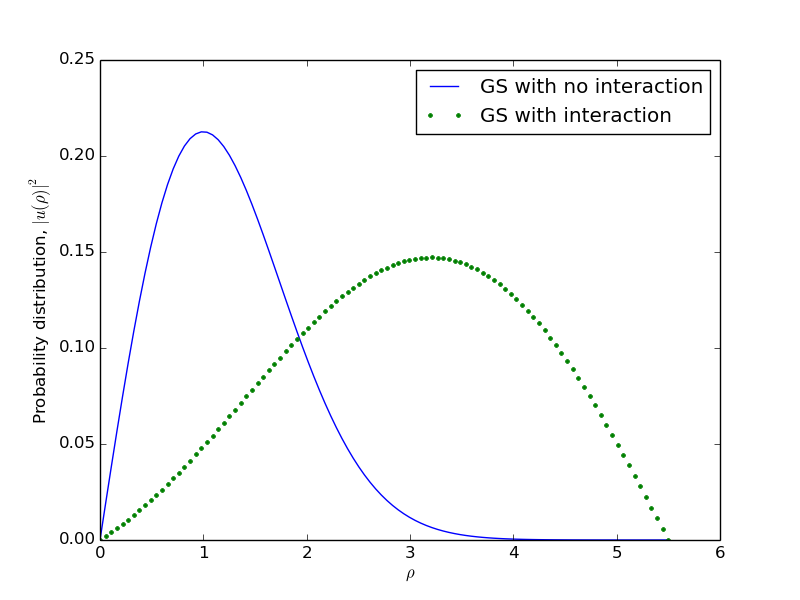
\includegraphics[width=\linewidth]{groundstates1.png}
	\caption{GS of the one-electron - and two-electron system.}
	\label{gs1}
	\end{figure}

\begin{figure}[H]
	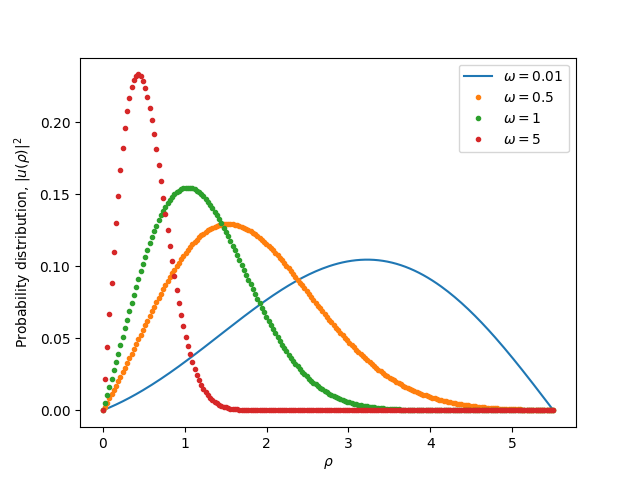
\includegraphics[width=\linewidth]{groundstates4.png}
	\caption{GS of the two-electron system for different frequencies $\omega$.}
	\label{gs4}
\end{figure}

	\section{Discussion}
	\subsection{The Algorithm}
	From table \ref{tab1} it becomes very clear that, as was mentioned in the section on implementation, that the Jacobi Rotation Method is highly inefficient. For only eight hundred points of integration the program has a run time of nearly eight minutes, and for a thousand points of integration the program uses an astounding 21 minutes to execute the method. One should also observe that the number of required iterations with respect to the given dimensionality $n$ follows $\mathcal{O}(1.8n^2)$
	\begin{figure}[H]
		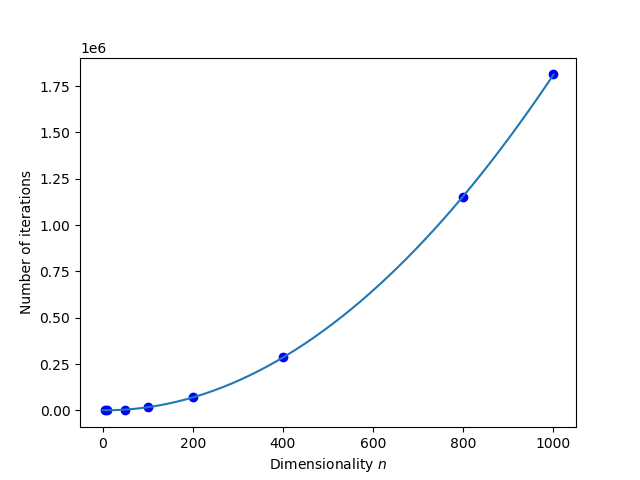
\includegraphics[width=\linewidth]{iterations.png}
		\label{iterations}
		\caption{A plot showing the evolution of number of iterations for a given $n$.}
	\end{figure}
	Here we have devised a library \texttt{numpy.polyfit()} do determine the gradient of the fitted polynomial.\\
	
	Although the program is numerically inefficient, it is nevertheless quite precise for low $n$, a conclusion we draw from having used the test function \texttt{TEST\_eigval()} to ensure that our computed eigenvalues are comparable to a benchmark tester using Armadillo's \texttt{eig\_sym()} with a given tolerance. 
	\subsection{The Physical Systems}
	Figure \ref{gs1} describes the physical state of a one-electron - and a two-electron system. Each plot describes the \emph{radial probability distribution} of the systems. We see that, for one electron in a 3D harmonic oscillator, the distribution is much sharper than it is for two electrons, meaning that a single electron is more localized than a system consisting of two.\\
	
	In figure \ref{gs4} we see plots of the ground state in a 3D harmonic oscillator occupied by two electrons and how the radial probability distribution changes as the oscillator frequency increases. Higher frequencies localizes the electrons more as seen by the smaller distributions, whilst lower frequencies results in a much larger distribution. One should from this conclude that higher frequencies causes the two electrons to have more well defined positions. 
	\section{Conclusive Remarks}
	In this study, we have found and presented that the Jacobi Rotation Method is a highly inefficient eigenvalue solver using a total number of iterations following $\mathcal{O}(1.8n^2)$ as a result of having to perform iterative transformations on off-diagonal elements to diagonalize a matrix within a given tolerance. Nevertheless, the algorithm finds tolerably precise eigenvalues for low dimensions $n$. We have also used the eigenvalue solver practically to solve the Schrödinger equation for one and two electrons in an harmonic oscillator well, and have made to findings about such systems; for one, introducing two electrons causes wider distributions in their radial probabilities, and secondly that for a two-electron system, increasing the frequency of the oscillator results in a more well defined average position. 
	\section{References}
	Hjorth-Jensen, Morten. \textit{Computational Physics: Lecture Notes Fall 2015}. PDF file. August 2015. \url{https://github.com/CompPhysics/ComputationalPhysics/blob/master/doc/Lectures/lectures2015.pdf}
\end{document}
